\documentclass{llncs}

\usepackage{amsmath} % for equation*
\usepackage{wasysym} % for \Box
\usepackage{color}
\usepackage{hyperref}
\usepackage{graphicx}
\definecolor{darkgreen}{rgb}{0,0.7,0}

\newcommand{\myspace}[0]{\vspace*{0.25cm}}

% Fix link colors
\hypersetup{
  colorlinks = true,
  linkcolor=red,
  citecolor=red,
  urlcolor=blue,
  linktocpage % so that page numbers are clickable in toc
}


\newcommand{\answer}[1]{{\color{red}\textit{#1}\color{black}}}
\title{COMP 445 -- Theoretical Assignment 1 (TA1)\\ Winter 2018}

\author{Tristan Glatard\\
  \href{mailto:tristan.glatard@concordia.ca}{tristan.glatard@concordia.ca}
}

\institute{Concordia University\\
  Department of Computer Science and Software Engineering}

\begin{document}

\maketitle

\section*{Instructions}

\begin{itemize}
\item Please submit your assignment  as a pdf file on Moodle. The name of the pdf file must contain your name and student id. 
\item All questions will receive equal points.
\item Each question may have zero, one, or more than one
  correct choices.
\item Wrong answers will be penalized with negative
  points.
\item Partial answers will not
  receive any point.
\item Blank answers (no answer) will not be penalized.
\end{itemize}

\hrulefill\\

\myspace

\myspace

Student ID: \dotfill

\myspace

\myspace

First Name / Last Name: \dotfill

\myspace

\myspace

Signature: \dotfill

\myspace

\myspace

\hrulefill

\newpage

\section*{Introduction}

\paragraph{\textbf{Q1:}} A protocol of the application layer is implemented:\\

\begin{tabular}{ccl}
  a) & $\Box$ & At the network core. \\
  \\
  b) & $\CheckedBox$ & At the network edge. \\
  \\
  c) & $\Box$ & Both at the network core and at the network edge. 
\end{tabular}

\answer{The application and transport layers are both implemented only at
  the network edge. It means that they are only implemented in end
  systems but not in routers. See slide 62 in Chapter 1.}

\paragraph{\textbf{Q2:}} Consider two hosts A and B connected through a single router X (the
  network looks like A -- X -- B). Assume that the link between A and
  X is of capacity $R_{A-X}$=8~Gbps and the link between X and B is of
  capacity $R_{X-B}$=16~Gbps. What is the time required for N=5
  packets of size L=1~MB to be delivered from A to B, assuming that all
  delays except the transmission delay are negligible? We assume that 1~Gb=1000~Mb.\\
  
\begin{tabular}{ccl}
  a) & $\CheckedBox$ & 5.5~ms\\
  \\
  b) & $\Box$ & 7.5~ms\\
  \\
  c) & $\Box$ & 1.5~ms\\
  \\
  d) & $\Box$ & None of the above.
\end{tabular}

\answer{ The delivery time is the sum of (1) the transmission delay
  \underline{of the last packet} from A to X and (2) the transmission delay
  \underline{of the last packet} from X to B.
\begin{itemize}
 \item Transmission delay from A to X: $t_{A-X}=N\frac{L}{R_{A-X}}$ (N-1 packets have to be transmitted before the last packet can be transmitted).
 \item Transmission delay from X to B: $t_{X-B}=\frac{L}{R_{X-B}}$ (when the last packet arrives in X, the first N-1 have already been transmitted since $R_{X-B}>R_{A-X}$).
 \item See slides 45-47 in Chapter 1.
\end{itemize}
}

\paragraph{\textbf{Q3:}} Starting from the same network as in the previous question, we now assume that propagation delays are not negligible:
\begin{itemize}
\item A and X are connected by a 5000-km link ($l_{A-X}$=5000~km) where the propagation speed is s=$10^8$~m/s.
\item B and X are connected by a 20-km link ($l_{X-B}$=20~km) where the propagation speed is s=$10^8$~m/s.
\end{itemize}
What is the new delivery time between A and B for the same N=5 packets?\\

\begin{tabular}{ccl}
  a) & $\Box$ & 45.7~ms\\
  \\
  b) & $\Box$ & 55.5~ms \\
  \\
  c) & $\Box$ & 51.5~ms\\
  \\
  d) & $\CheckedBox$ & 55.7~ms
\end{tabular}


\answer{The propagation delay adds to the transmission time. The new delivery time is: $t_{A-X}+t_{X-B}+\frac{l_{A-X}}{s}+\frac{l_{X-B}}{s}$.
See slide 45 in Chapter 1. 
}

\paragraph{\textbf{Q4:}} In the Internet protocol stack, the transport layer can directly use services from:\\

\begin{tabular}{ccl}
  a) & $\Box$ & The application layer.\\
  \\
  b) & $\CheckedBox$ & The network layer.\\
  \\
  c) & $\Box$ & The link layer.\\
  \\
  d) & $\Box$ & All of the above.
\end{tabular}

\answer{In the layer model, a layer only uses services from the layer just below. See slide 58 in Chapter 1. }

\paragraph{\textbf{Q5:}} What is the probability that more than 5 users are active at the same time in a network of 15 users where each user is active 20\% of the time?\\

\begin{tabular}{ccl}
  a) & $\Box$ & 1\\
  \\
  b) & $\Box$ & 0.6\\
  \\
  c) & $\Box$ & 0.04\\
  \\
  d) & $\CheckedBox$ & 0.06
\end{tabular}

\answer{
  $P=\sum_{i=6}^{15}{\binom {15}i 0.2^{i}0.8^{(15-i)}}$. See slide 30 in Chapter 1.
}

\section*{Application layer}

\paragraph{\textbf{Q6:}}
The content below was captured using
Wireshark:\\
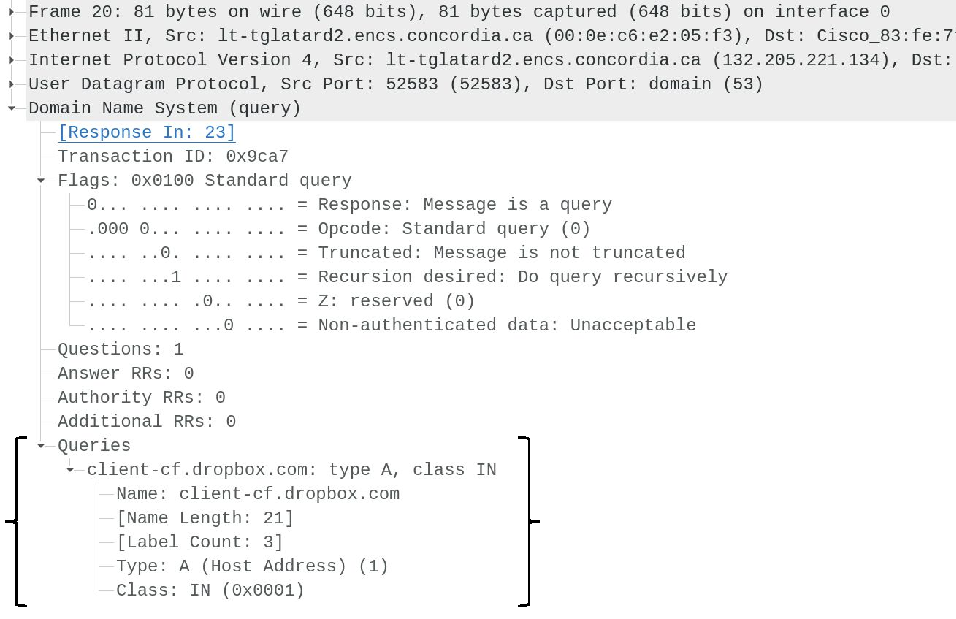
\includegraphics[width=\textwidth]{dns.png}
This trace contains:\\

\begin{tabular}{ccl}
  a) & $\Box$ & An HTTP request encapsulated in a DNS query.\\
  \\
  b) & $\Box$ & A DNS query encapsulated in a TCP segment.\\
  \\
  c) & $\Box$ & An IP datagram encapsulated in a UDP datagram.\\
  \\
  d) & $\CheckedBox$ & A DNS query encapsulated in a UDP datagram.
\end{tabular}

\answer{Wireshark traces are read from bottom to top. DNS (Domain Name
  System) is an application-level protocol therefore it has to use a
  transport-level protocol which happens to be UDP (User Datagram
  Protocol) here. IP datagrams could never be encapsulated in UDP datagrams
  since IP belongs to a lower layer than UDP. HTTP requests could
  never be encapsulated in DNS queries since both protocols are
  application-level.}

\paragraph{\textbf{Q7:}} Among the following HTTP methods, which one(s) may be used to upload a file to a
Web server?\\

\begin{tabular}{ccl}
  a) & $\Box$ & GET\\
  \\
  b) & $\CheckedBox$ & POST\\
  \\
  c) & $\CheckedBox$ & PUT\\
  \\
  d) & $\Box$ & HEAD\\
\end{tabular}

\answer{See slides 29-30 in Chapter 2.}

\paragraph{\textbf{Q8:}} Among the following protocols, which one(s) are \textbf{not} involved in the retrieval of the Web page at URL \texttt{http://www.concordia.ca/} with a Web browser?\\

\begin{tabular}{ccl}
  a) & $\Box$ & TCP\\
  \\
  b) & $\Box$ & DNS\\
  \\
  c) & $\Box$ & HTTP\\
  \\
  d) & $\CheckedBox$ & SMTP\\
\end{tabular}

\answer{Before the communication can be initiated, the IP address of
  \texttt{www.concordia.ca} has to be looked up, which is done using
  DNS. The connection is then established using TCP. Finally, the
  webpage is requested using HTTP. SMTP is an email protocol which has
  nothing to do with the Web.}

\paragraph{\textbf{Q9:}} DNS may be used to retrieve the name of the email server of a specific domain:\\

\begin{tabular}{ccl}
  a) & $\Box$ & by querying records of type CNAME.\\
  \\
  b) & $\Box$ & by querying records of type NS.\\
  \\
  c) & $\Box$ & through any type of iterated query.\\
  \\
  d) & $\Box$ & through any type of recursive query.\\
\end{tabular}

\answer{None of the options are correct. a) CNAME records associate
  names with canonical names, they are used to lookup aliases. b) NS
  records associate domain names with host names, they are used to
  lookup name servers. c) and d) Iterated or recursive queries can be
  used for any type of query but they don't preclude any particular
  record type. Email servers can be retrieved by querying for MX
  records. See slide 66 in Chapter 2.}

\paragraph{\textbf{Q10:}} SMTP is:\\

\begin{tabular}{ccl}
  a) & $\CheckedBox$ & a push protocol.\\
  \\
  b) & $\Box$ & a deprecated protocol.\\
  \\
  c) & $\Box$ & a transport protocol (a protocol belonging to the transport layer).\\
  \\
  d) & $\CheckedBox$ & a text (ASCII) protocol.\\
\end{tabular}

\answer{See slides 47 and 51 in Chapter 2. SMTP is still used in all
  email communications -- it is not deprecated. It is an application
  protocol, not a transport one.}

\end{document}
